%% =============================================================================
%% EVALUATION
%% =============================================================================

\section{Evaluation} \label{sec:evaluation}

A chat-first system must demonstrate that LLMs can reliably select
appropriate tools and extract correct parameters. This section evaluates
LLM performance across single-turn tool selection, multi-turn conversations,
naturalistic prompts, parameter extraction, interpretation accuracy, and
out-of-scope detection, using 10 models ranging from 3B to 72B parameters.

\subsection{Tool selection evaluation}

We evaluated LLM performance on 87 test cases spanning regression, panel data,
causal inference, discrete choice, time series, hypothesis testing, machine
learning, and visualization. Each case presents a natural language prompt; the
model must select the appropriate tool from the \pkg{prompt2analytics} schema.
Responses are scored as exact (correct tool), acceptable (valid alternative),
category (correct domain, wrong method), or failed. Accuracy is computed as
(exact + acceptable) / total.

\subsubsection{Evaluation methodology and reproducibility}

All evaluations used temperature $= 0$ for deterministic outputs. The system
prompt instructs the model to select a single tool from the provided MCP schema
and return a structured JSON response with tool name and parameters. The
complete system prompt is provided in the supplementary materials file
\code{llm\_eval\_prompts.txt}; the summary form is:

\begin{quote}
\small
``You are an assistant that selects statistical tools. Given a user request,
choose exactly one tool from the available schema and provide the required
parameters. Respond with valid JSON containing `tool\_name' and `parameters'.''
\end{quote}

\noindent Table~\ref{tab:model-versions} lists the model versions used for
evaluation. API-served models may change over time, so exact replication of
cloud-hosted results may not be possible. Local models evaluated via Ollama
use fixed quantization levels, improving reproducibility.

\begin{table}[htbp]
\centering
\begin{threeparttable}
\caption{Model versions used for evaluation (accessed January 2026)}
\label{tab:model-versions}
\small
\begin{tabular}{lll}
\toprule
Model & Version ID & Provider \\
\midrule
Claude 3.5 Haiku & \code{claude-3-5-haiku-20241022} & Anthropic API \\
Claude 3.5 Sonnet & \code{claude-3-5-sonnet-20241022} & Anthropic API \\
GPT-4o & \code{gpt-4o-2024-08-06} & OpenAI API \\
GPT-4o-mini & \code{gpt-4o-mini-2024-07-18} & OpenAI API \\
GPT-4.1 Nano & \code{gpt-4.1-nano-2025-04-14} & OpenAI API \\
Llama 3.1 8B & Q4\_K\_M quantization & Ollama (local) \\
Llama 3.3 70B & Q4\_K\_M quantization & Ollama (local) \\
Qwen 2.5 7B & Q4\_K\_M quantization & Ollama (local) \\
Qwen 2.5 72B & Q4\_K\_M quantization & Ollama (local) \\
Ministral 3B & Q4\_K\_M quantization & Ollama (local) \\
\bottomrule
\end{tabular}
\end{threeparttable}
\end{table}

\begin{figure}[htbp]
\centering
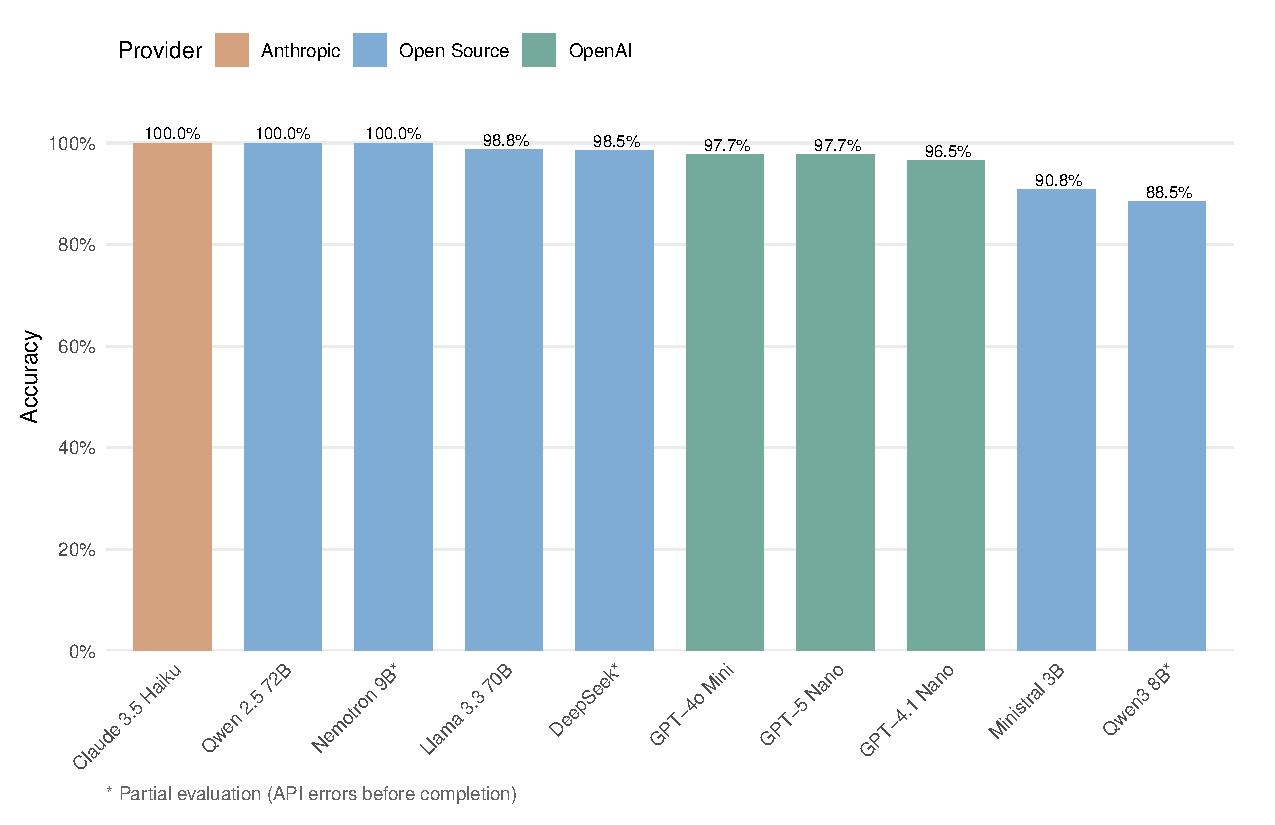
\includegraphics[width=0.85\textwidth]{figures/fig_accuracy_comparison}
\caption{Tool selection accuracy across models. Accuracy is computed as
(exact + acceptable matches) / total tests. All models were evaluated on
the complete 87-test benchmark. Claude 3.5 Haiku and Qwen 2.5 72B achieve
perfect accuracy; even the smallest model (Ministral 3B at 3 billion
parameters) exceeds 90\%.}
\label{fig:accuracy-comparison}
\end{figure}

Figure~\ref{fig:accuracy-comparison} presents overall accuracy by model.
The results demonstrate that tool selection---unlike code generation---is
achievable even by smaller models. Claude 3.5 Haiku and Qwen 2.5 72B
(an open-source model) achieve 100\% accuracy. Notably, Ministral 3B,
a model small enough to run on consumer hardware with only 6~GB VRAM,
achieves 90.8\% accuracy, making it viable for local deployment scenarios
where hardware constraints preclude larger models.

\begin{figure}[htbp]
\centering
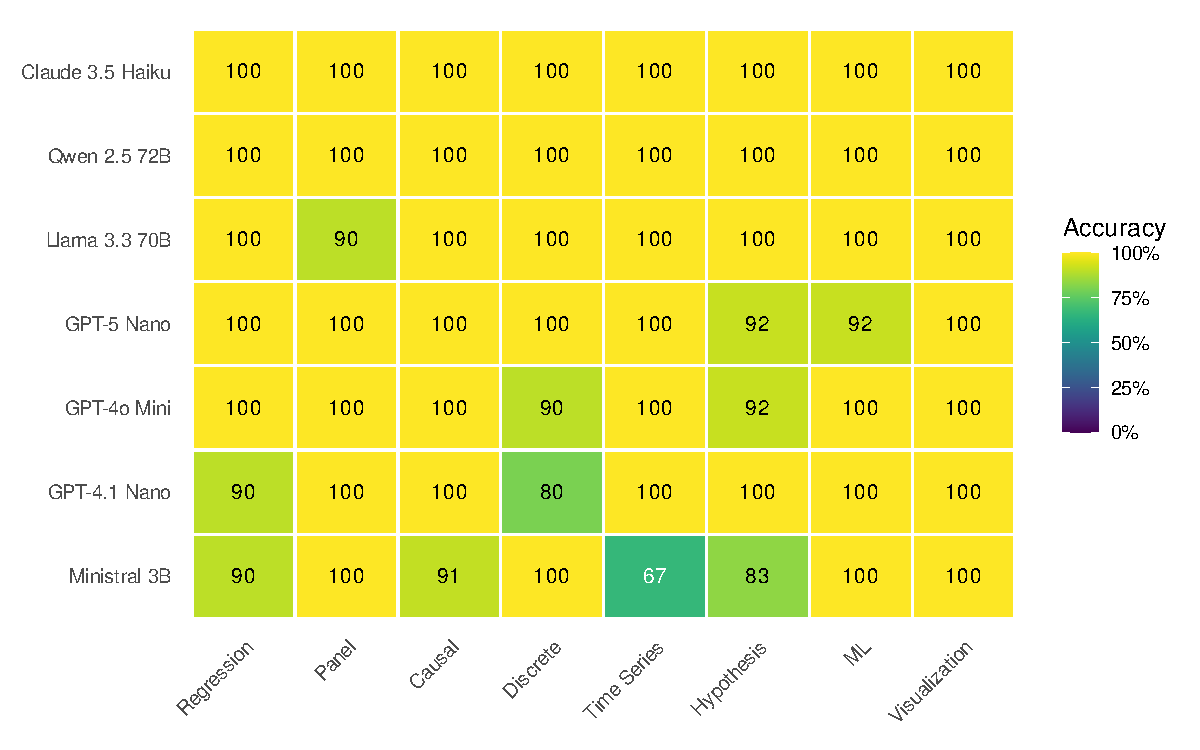
\includegraphics[width=0.95\textwidth]{figures/fig_accuracy_by_category}
\caption{Accuracy breakdown by test category. Darker cells indicate lower
accuracy. Most models achieve 100\% on standard categories; errors
concentrate in edge cases involving ambiguous method selection
(e.g., logit with fixed effects vs.\ FEGLM).}
\label{fig:accuracy-category}
\end{figure}

Figure~\ref{fig:accuracy-category} shows accuracy by category. Performance
is uniformly high across most categories, with errors concentrated in
edge cases requiring fine distinctions between related methods. For instance,
Ministral 3B shows lower accuracy on time series (66.7\%) where distinguishing
between VAR, VARMA, and VECM specifications proves challenging for the
smaller model. Specific confusion patterns include: selecting VAR when VECM
is appropriate (failing to recognize cointegration requirements), choosing
ARIMA for multivariate series that require VAR, and defaulting to simpler
univariate methods when the prompt describes multiple interrelated series.

Tables~\ref{tab:model-summary} and \ref{tab:category-accuracy} in
Appendix~\ref{app:llm-eval} provide detailed breakdowns of model
performance and per-category accuracy. Appendix~\ref{app:latency}
reports API response latencies, though these figures reflect cloud-hosted
inference and do not directly apply to local deployment scenarios.

\subsection{Extended robustness evaluation}

The single-turn evaluation on curated prompts establishes baseline tool selection
accuracy but leaves several questions unanswered: How do models perform across
multi-turn conversations? Do they handle naturalistic language with typos and
informal phrasing? Can they extract parameters correctly and interpret results
accurately? To address these gaps, we conducted an extended evaluation across
five dimensions using the same 10 models.

\textbf{Multi-turn conversations.} We constructed 20 multi-turn conversations
totaling 72 turns, where each turn builds on previous context (e.g., ``Now use
robust standard errors instead''). The results surprised us: accuracy depends
heavily on what goes into the conversation history. When models can see their
previous tool calls and results, they correctly resolve references like ``those
results'' or ``the previous model.'' Without this context, they cannot.
GPT-4o-mini with full context achieves 97.2\% turn accuracy and 90\% conversation
completion. Qwen3 8B reaches 83.3\% and 60\%. But strip out the tool call
history, and accuracy drops to 47--60\% across the board. The lesson is simple:
conversation history must include tool invocations, not just the text exchange.

\textbf{Naturalistic prompts.} We tested 99 prompts featuring realistic
variations: typos (``regresion''), informal language (``run a quick OLS''),
domain jargon (``estimate the ATT''), verbose descriptions, and ambiguous
phrasing. Accuracy ranges from 58--70\%, with Claude 3.5 Haiku achieving
the highest robustness (69.7\%). Models handle typos well (65--69\% accuracy)
but struggle more with ambiguous specifications (42--58\%).

\textbf{Parameter extraction.} Beyond tool selection, LLMs must extract
variable names, options, and modifiers. We evaluated 49 parameter extraction
tasks, measuring precision, recall, and F1 score. Average F1 ranges from
70--90\% across models, with GPT-4o-mini achieving the highest score (89.6\%).
The dominant error is omission of optional parameters (e.g., robust SE type,
clustering specification); wrong values account for fewer than 5\% of errors.

\textbf{Interpretation accuracy.} We evaluated whether models correctly
interpret statistical output across 26 test cases covering coefficient
interpretation, significance testing, and diagnostic results. Models
achieve 68--87\% accuracy, with GPT-4.1 Nano performing best (87.2\%).
Errors typically involve misinterpreting log-transformed coefficients
or overlooking important caveats about statistical significance.

\textbf{Out-of-scope detection.} When users request methods outside the
implemented set (e.g., Bayesian inference, structural equation modeling), the system should
either decline gracefully or suggest alternatives. Detection rates range
from 40--60\%, with most undetected cases resulting in selection of a
superficially similar but incorrect method.

Table~\ref{tab:extended-eval-summary-main} summarizes the results.

\begin{table}[htbp]
\centering
\begin{threeparttable}
\caption{Extended evaluation results: the gap between controlled benchmarks and realistic use}
\label{tab:extended-eval-summary-main}
\small
\begin{tabular}{lcc}
\toprule
Metric & Range & Best Model \\
\midrule
Single-turn tool selection & 90.8--100\% & Qwen 2.5 72B, Claude 3.5 Haiku \\
Multi-turn accuracy & 47--97\% & GPT-4o-mini (97.2\%) \\
Conversation completion & 15--90\% & GPT-4o-mini (90\%) \\
Naturalistic prompt robustness & 58--70\% & Claude 3.5 Haiku (69.7\%) \\
Parameter extraction F1 & 70--90\% & GPT-4o-mini (89.6\%) \\
Interpretation accuracy & 68--87\% & GPT-4.1 Nano (87.2\%) \\
Out-of-scope detection & 40--60\% & Llama 3.3 70B (60\%) \\
\bottomrule
\end{tabular}
\begin{tablenotes}\small
\item \emph{Note:} Multi-turn results reflect V3 evaluation with enhanced
context (tool calls in history). Values show range across evaluated models.
\end{tablenotes}
\end{threeparttable}
\end{table}

Figure~\ref{fig:robustness-radar} in Appendix~\ref{app:extended-eval}
visualizes the multi-dimensional performance profile for each model.

\textbf{What this means.} Context management matters more than model choice.
With tool calls in history, even Qwen3 8B (an 8-billion parameter open model)
hits 83\% multi-turn accuracy. Without it, 70-billion parameter models struggle
to break 60\%. Parameter extraction is moderate (F1 of 70--90\%), with
errors concentrated in omission of optional parameters rather than wrong
values. Users should still verify extracted parameters before trusting
results. For practical deployment: include tool calls in conversation
history, and verify parameters before interpreting output.

\subsection{Failure modes}

Understanding system behavior under failure conditions is essential for
informed use. Three categories of failure merit discussion.

\textbf{Method misselection.}
When the LLM selects an inappropriate statistical method, the system
proceeds with the selected method and returns results. Users must
recognize the mismatch between request and execution. Common patterns
include ambiguous specifications (``regression with firm effects'' could
invoke OLS, fixed effects, or random effects), similar method confusion
(VAR/VECM/VARMA), and capability boundary cases where requests for
unimplemented methods map to superficially similar available tools.
Users can mitigate misselection by specifying methods explicitly
rather than describing goals abstractly.

\textbf{Parameter extraction errors.}
Even when the correct method is selected, the LLM may extract incorrect
parameters: variable names that do not exist in the dataset, omitted
specification options (robust SEs, clustering), or incorrect defaults.
The dataset schema---column names and types---is provided to the LLM as
context, which substantially reduces variable name errors. Explicit
phrasing (``with HC1 robust standard errors'') yields more reliable
extraction than implicit expectations.

\textbf{Categorical variable handling.}
Categorical (string) variables are automatically converted to dummy variables
using treatment coding (one level omitted as reference). The system detects
string columns, creates indicator variables, reports the reference category,
and warns when categorical variables have many levels ($>50$).
